\providecommand{\main}{..}
\documentclass[\main/main.tex]{subfiles}

\graphicspath{ {\main/chapters/circuiti/}} 

\begin{document}

\section{MOS Intro}

I MOS (Metal Oxide Semiconductor) sono dei tripoli a base di semiconduttori.

Sono ricavati da un substrato di semicoduttore drogato di un tipo in cui si realizzano due piazzole drogate in modo opposto e tra di esse vi si crea uno strato di ossido che funge da dielettrico.
Sopra alle piazzole ed al ossido si relizzano dei contatti metallici per poter collegare il MOS ai vari circuiti.

A seconda che si droghino le piazzole di tipo N o di tipo P si distinguono in NMOS e PMOS i quali sono sostanzialmente duali nel funzionamento.

I 

\begin{figure}[H]
\center
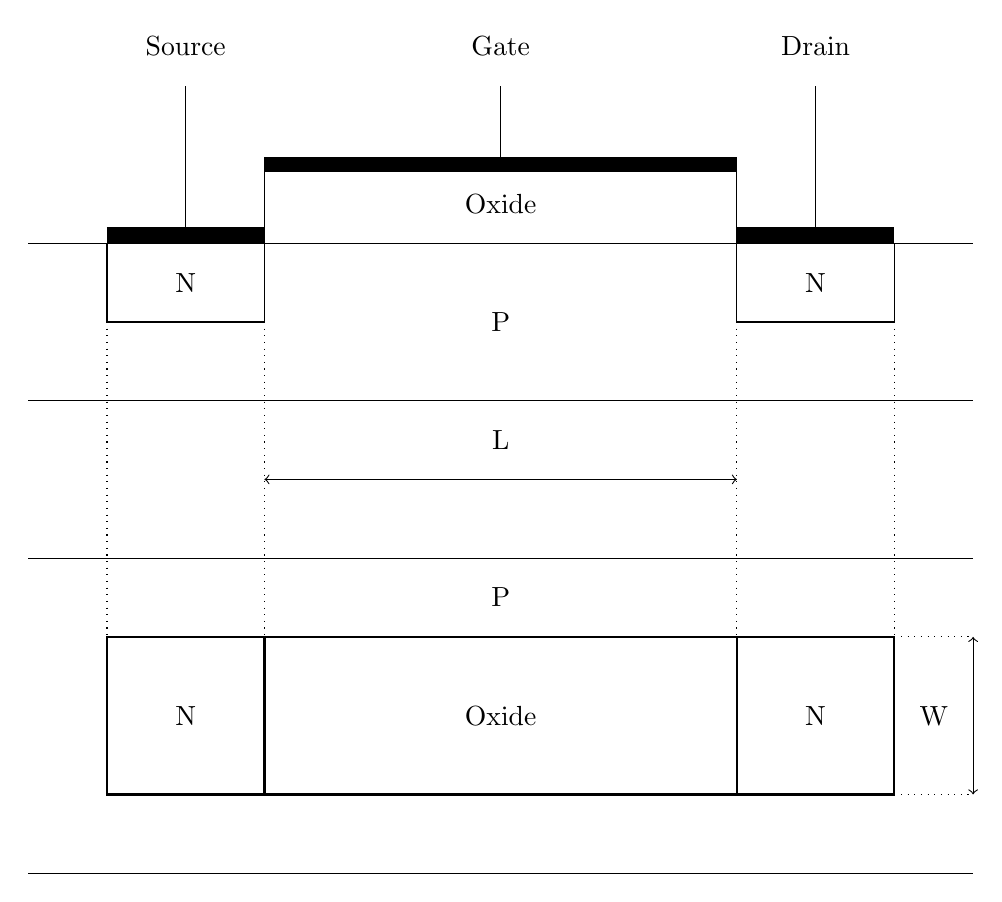
\begin{tikzpicture}
% Silicon Top
\draw (0,0)  -- (12,0);
\draw (0,-2)  -- (12,-2);

% Piazzola Source
\draw (1,0)  -- (1,-1);
\draw (1,-1) -- (3,-1);
\draw (3,-1) -- (3,0);
\draw [line width=0.2cm] (1,0.1)  -- (3,0.1);

% Piazzola Drain
\draw (9,0)  -- (9,-1);
\draw (9,-1) -- (11,-1);
\draw (11,-1) -- (11,0);
\draw [line width=0.2cm] (9,0.1)  -- (11,0.1);

% Gate
\draw (3,0)  -- (3,1);
\draw [line width=0.2cm] (3,1)  -- (9,1);
\draw (9,1)  -- (9,0);

% Gate Terminal
\draw (6,1) -- (6,2);
\node[] at (6,2.5) {Gate};

% Source Terminal
\draw (10,0) -- (10,2);
\node[] at (10,2.5) {Drain};

% Drain Terminal
\draw (2,0) -- (2,2);
\node[] at (2,2.5) {Source};

% Letters
\node[] at (2,-0.5) {N};
\node[] at (10,-0.5) {N};
\node[] at (6,-1) {P};
\node[] at (6,0.5) {Oxide};

%SEZIONE DAL ALTO

% Silicon Top
\draw (0,-4)  -- (12,-4);
\draw (0,-8)  -- (12,-8);

%Mos top
\draw [fill=white, thick] (1,-5) rectangle (3,-7);
\draw [fill=white, thick] (3,-5) rectangle (9,-7);
\draw [fill=white, thick] (9,-5) rectangle (11,-7);

% Letters
\node[] at (2,-6) {N};
\node[] at (10,-6) {N};
\node[] at (6,-4.5) {P};
\node[] at (6,-6) {Oxide};

% L
\draw [<->] (3,-3) -- (9,-3);
\draw[dotted] (3,-1) -- (3,-5);
\draw[dotted] (9,-1) -- (9,-5);
\node[] at (6,-2.5) {L};

% W
\draw [<->] (12,-7) -- (12,-5);
\draw[dotted] (11,-7) -- (12,-7);
\draw[dotted] (11,-5) -- (12,-5);
\node[] at (11.5,-6) {W};

% projection dot
\draw[dotted] (1,-1) -- (1,-5);
\draw[dotted] (11,-1) -- (11,-5);

\end{tikzpicture}
\caption{Vista in sezione e dal alto di un NMOS}
\end{figure}


Definisco due caratteristiche del MOS:
\[K_n' = \frac{1}{2} \mu_n C_{ox}'\]
\[K_n = K_n' \left(\frac{W}{L}\right) = \frac{1}{2} \mu_n C_{ox}'\left(\frac{W}{L}\right)\]
\begin{align*}
\mu_n &\text{ e' la costante di mobilita' delle cariche libere}\\
C_{ox}' &\text{ e' la capacita' del condesatore che si forma tra il gate ed il canale}\\
W &\text{ e' la larghezza del canale}\\
L &\text{ e' la lunghezza del canale}
\end{align*}
\clearpage
\subsection{Regimi di Funzionamento di un MOS}
In realta' nelle zone di confine tra le piazzole ed il substrato si forma uno strato neutro poiche' a contatto da una parte con una zona drogata positivamente ed una drogata negativamente.

Quindi una immagine piu' reale del MOS e':

\begin{figure}[H]
\center
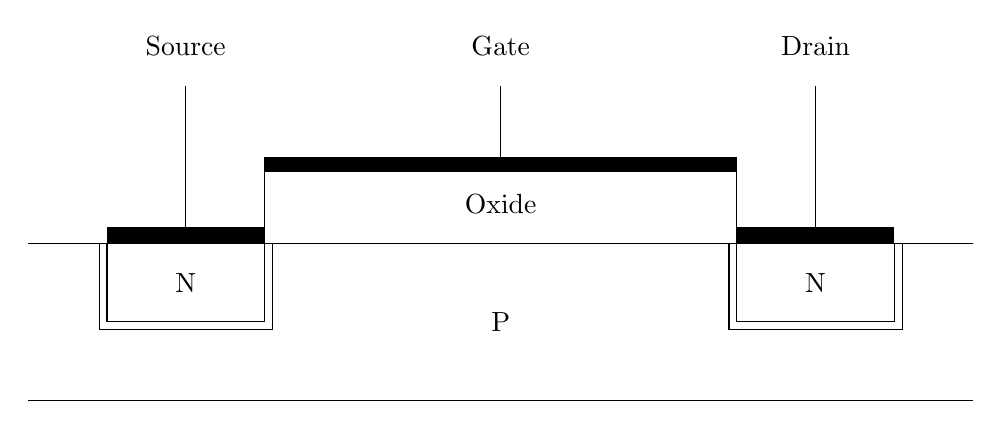
\begin{tikzpicture}
% Silicon Top
\draw (0,0)  -- (12,0);
\draw (0,-2)  -- (12,-2);

% Piazzola Source
\draw (1,0)  -- (1,-1);
\draw (1,-1) -- (3,-1);
\draw (3,-1) -- (3,0);
\draw [line width=0.2cm] (1,0.1)  -- (3,0.1);
\draw (0.9,0)  -- (0.9,-1.1);
\draw (0.9,-1.1) -- (3.1,-1.1);
\draw (3.1,-1.1) -- (3.1,0);

% Piazzola Drain
\draw (9,0)  -- (9,-1);
\draw (9,-1) -- (11,-1);
\draw (11,-1) -- (11,0);
\draw [line width=0.2cm] (9,0.1)  -- (11,0.1);
\draw (8.9,0)  -- (8.9,-1.1);
\draw (8.9,-1.1) -- (11.1,-1.1);
\draw (11.1,-1.1) -- (11.1,0);

% Gate
\draw (3,0)  -- (3,1);
\draw [line width=0.2cm] (3,1)  -- (9,1);
\draw (9,1)  -- (9,0);

% Gate Terminal
\draw (6,1) -- (6,2);
\node[] at (6,2.5) {Gate};

% Source Terminal
\draw (10,0) -- (10,2);
\node[] at (10,2.5) {Drain};

% Drain Terminal
\draw (2,0) -- (2,2);
\node[] at (2,2.5) {Source};

% Letters
\node[] at (2,-0.5) {N};
\node[] at (10,-0.5) {N};
\node[] at (6,-1) {P};
\node[] at (6,0.5) {Oxide};

\end{tikzpicture}
\caption{Sezione di un NMOS con le zone neutre a vista}
\end{figure}

Normalmente nelle reallizzazzioni pratiche il substrato e' collegato al source

\begin{figure}[H]
\center
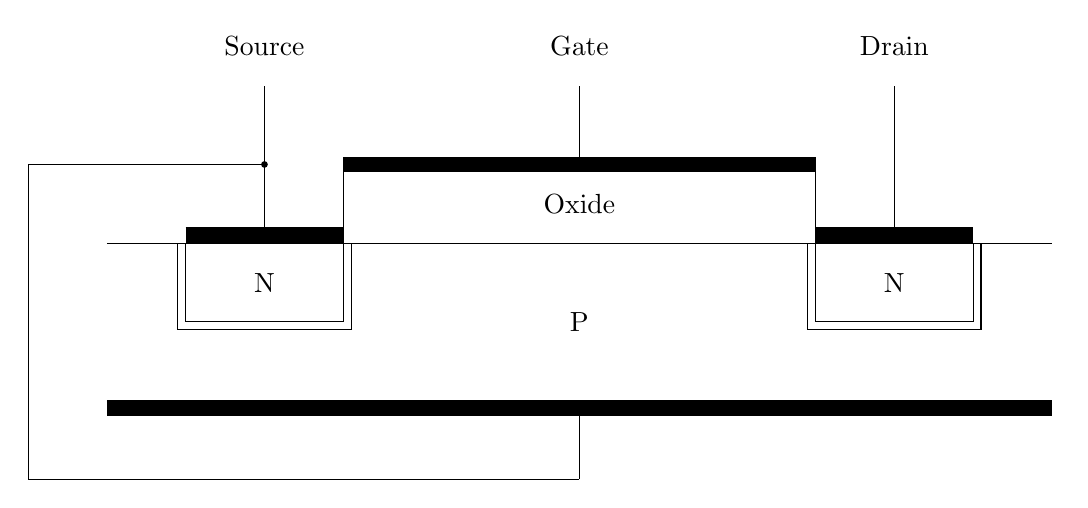
\begin{tikzpicture}
% Silicon Top
\draw (0,0)  -- (12,0);
\draw (0,-2)  -- (12,-2);
\draw [line width=0.2cm] (0,-2.1)  -- (12,-2.1);

% Piazzola Source
\draw (1,0)  -- (1,-1);
\draw (1,-1) -- (3,-1);
\draw (3,-1) -- (3,0);
\draw [line width=0.2cm] (1,0.1)  -- (3,0.1);
\draw (0.9,0)  -- (0.9,-1.1);
\draw (0.9,-1.1) -- (3.1,-1.1);
\draw (3.1,-1.1) -- (3.1,0);
\draw (6,-2) -- (6,-3);
\draw (6,-3) -- (-1,-3);
\draw (-1,-3) -- (-1,1);
\draw (-1,1) -- (2,1);

\filldraw [black] (2,1) circle (1pt) node[below, black] {};


% Piazzola Drain
\draw (9,0)  -- (9,-1);
\draw (9,-1) -- (11,-1);
\draw (11,-1) -- (11,0);
\draw [line width=0.2cm] (9,0.1)  -- (11,0.1);
\draw (8.9,0)  -- (8.9,-1.1);
\draw (8.9,-1.1) -- (11.1,-1.1);
\draw (11.1,-1.1) -- (11.1,0);

% Gate
\draw (3,0)  -- (3,1);
\draw [line width=0.2cm] (3,1)  -- (9,1);
\draw (9,1)  -- (9,0);

% Gate Terminal
\draw (6,1) -- (6,2);
\node[] at (6,2.5) {Gate};

% Source Terminal
\draw (10,0) -- (10,2);
\node[] at (10,2.5) {Drain};

% Drain Terminal
\draw (2,0) -- (2,2);
\node[] at (2,2.5) {Source};

% Letters
\node[] at (2,-0.5) {N};
\node[] at (10,-0.5) {N};
\node[] at (6,-1) {P};
\node[] at (6,0.5) {Oxide};

\end{tikzpicture}
\caption{Sezione di un NMOS con source collegato al substrato}
\end{figure}


Ora se imponiamo a massa il Source ed il Drain ed iniziamo ad aumentare il potenziale ai capi del Gate si iniziano ad accumulare cariche sul Gate che come un condensatore attrae cariche opposte, sotto l'ossido, iniziando a formare una zona neutra.

Il MOS continua a rimaene spento e non vi puo' essere conduzione tra Source e Drain.

In realta' vi e' una piccola corrente di cross-conduzione ma tranquillamente approssimabile a 0 poiche' di diversi ordini di grandezza piu' piccola di quelle degli agltri regimi di funzionamento.

\[I_{DS} = 0\]

\begin{figure}[H]
\center
\begin{circuitikz}
% Silicon Top
\draw (0,0)  -- (12,0);
\draw (0,-2)  -- (12,-2);
\draw [line width=0.2cm] (0,-2.1)  -- (12,-2.1);

% Piazzola Source
\draw (1,0)  -- (1,-1);
\draw (1,-1) -- (3,-1);
\draw (3,-1) -- (3,0);
\draw [line width=0.2cm] (1,0.1)  -- (3,0.1);
\draw (0.9,0)  -- (0.9,-1.1);
\draw (0.9,-1.1) -- (3.1,-1.1);
\draw (3.1,-1.1) -- (3.1,-0.1);

% Piazzola Drain
\draw (9,0)  -- (9,-1);
\draw (9,-1) -- (11,-1);
\draw (11,-1) -- (11,0);
\draw [line width=0.2cm] (9,0.1)  -- (11,0.1);
\draw (8.9,-0.1)  -- (8.9,-1.1);
\draw (8.9,-1.1) -- (11.1,-1.1);
\draw (11.1,-1.1) -- (11.1,0);
\draw (6,-2) -- (6,-3);
\draw (6,-3) -- (-1,-3);
\draw (-1,-3) -- (-1,1);
\draw (-1,1) -- (2,1);

\filldraw [black] (2,1) circle (1pt) node[below, black] {};

% Gate
\draw (3,0)  -- (3,1);
\draw [line width=0.2cm] (3,1)  -- (9,1);
\draw (9,1)  -- (9,0);
\draw (3.1,-0.1)  -- (8.9,-0.1);

% Gate Terminal
\draw (6,1) -- (6,2);
\node[] at (6,2.5) {Gate};

% Source Terminal
\draw (10,0) -- (10,3.5);
\node[] at (11,2.5) {Drain};

% Drain Terminal
\draw (2,0) -- (2,3.5);
\node[] at (1,2.5) {Source};

% Letters
\node[] at (2,-0.5) {N};
\node[] at (10,-0.5) {N};
\node[] at (6,-1) {P};
\node[] at (6,0.5) {Oxide};

\draw (6,2) to[american voltage source, v_<= $V_{GS}$] (2,2);

\filldraw [black] (2,2) circle (1pt) node[below, black] {};

\draw (2,3.5) -- (10,3.5);

\end{circuitikz}
\caption{Sezione di un NMOS al aumentare del potenziale sul Gate}
\end{figure}

Una volta che il Potenziale al Gate ha superato una Tensione di Soglia $V_t$ ( che e' una caratteritica del MOS) si inizia a formare un canale polarizzato come le piazzole il quale avendo cairche libere puo' essere attraversato da una corrente tra Source e Drain $I_{DS}$.

In questa situazione in cui vi e' il canale da entrambi i lati si dice che il MOS sta lavorando in regime Ohmmico.

\[I_{DS} = K_n \left[ 2 \left(V_{GS} - V_t \right)V_{DS} - V_{DS}^2 \right]\]

\begin{figure}[H]
\center
\begin{circuitikz}
% Silicon Top
\draw (0,0)  -- (12,0);
\draw (0,-2)  -- (12,-2);
\draw [line width=0.2cm] (0,-2.1)  -- (12,-2.1);

% Piazzola Source
\draw (1,0)  -- (1,-1);
\draw (1,-1) -- (3,-1);
\draw (3,-1) -- (3,-0.4);
\draw [line width=0.2cm] (1,0.1)  -- (3,0.1);
\draw (0.9,0)  -- (0.9,-1.1);
\draw (0.9,-1.1) -- (3.1,-1.1);
\draw (3.1,-1.1) -- (3.1,-0.5);

% Piazzola Drain
\draw (9,-0.4)  -- (9,-1);
\draw (9,-1) -- (11,-1);
\draw (11,-1) -- (11,0);
\draw [line width=0.2cm] (9,0.1)  -- (11,0.1);
\draw (8.9,-0.5)  -- (8.9,-1.1);
\draw (8.9,-1.1) -- (11.1,-1.1);
\draw (11.1,-1.1) -- (11.1,0);
\draw (6,-2) -- (6,-3);
\draw (6,-3) -- (-1,-3);
\draw (-1,-3) -- (-1,1);
\draw (-1,1) -- (2,1);

\filldraw [black] (2,1) circle (1pt) node[below, black] {};

% Gate
\draw (3,0)  -- (3,1);
\draw [line width=0.2cm] (3,1)  -- (9,1);
\draw (9,1)  -- (9,0);
\draw (3,-0.4)  -- (9,-0.4);
\draw (3.1,-0.5)  -- (8.9,-0.5);

% Gate Terminal
\draw (6,1) -- (6,2);
\node[] at (6,2.5) {Gate};

% Source Terminal
\draw (10,0) -- (10,3.5);
\node[] at (11,2.5) {Drain};

% Drain Terminal
\draw (2,0) -- (2,3.5);
\node[] at (1,2.5) {Source};

% Letters
\node[] at (2,-0.5) {N};
\node[] at (10,-0.5) {N};
\node[] at (6,-1) {P};
\node[] at (6,0.5) {Oxide};

\draw (6,2) to[american voltage source, v_<= $V_{GS}$] (2,2);

\filldraw [black] (2,2) circle (1pt) node[below, black] {};

\draw (2,3.5) -- (10,3.5);

\draw[dotted] (3,0) -- (3,-0.5);
\draw[dotted] (9,0) -- (9,-0.5);

\end{circuitikz}
\caption{Sezione di un NMOS al aumentare del potenziale sul Gate}
\end{figure}

Ora se impongo una tensione $V_{DS}$ il canale inizia ad essere attratto verso il drain quindi il canale non e' piu' parallelo al' ossido ma diventa.


\begin{figure}[H]
\center
\begin{circuitikz}
% Silicon Top
\draw (0,0)  -- (12,0);
\draw (0,-2)  -- (12,-2);
\draw [line width=0.2cm] (0,-2.1)  -- (12,-2.1);

% Piazzola Source
\draw (1,0)  -- (1,-1);
\draw (1,-1) -- (3,-1);
\draw (3,-1) -- (3,-0.6);
\draw [line width=0.2cm] (1,0.1)  -- (3,0.1);
\draw (0.9,0)  -- (0.9,-1.1);
\draw (0.9,-1.1) -- (3.1,-1.1);
\draw (3.1,-1.1) -- (3.1,-0.7);

% Piazzola Drain
\draw (9,-0.2)  -- (9,-1);
\draw (9,-1) -- (11,-1);
\draw (11,-1) -- (11,0);
\draw [line width=0.2cm] (9,0.1)  -- (11,0.1);
\draw (8.9,-0.3)  -- (8.9,-1.1);
\draw (8.9,-1.1) -- (11.1,-1.1);
\draw (11.1,-1.1) -- (11.1,0);
\draw (6,-2) -- (6,-3);
\draw (6,-3) -- (-1,-3);
\draw (-1,-3) -- (-1,1);
\draw (-1,1) -- (2,1);

\filldraw [black] (2,1) circle (1pt) node[below, black] {};

% Gate
\draw (3,0)  -- (3,1);
\draw [line width=0.2cm] (3,1)  -- (9,1);
\draw (9,1)  -- (9,0);
\draw (3,-0.6)  -- (9,-0.2);
\draw (3.1,-0.7)  -- (8.9,-0.3);

% Gate Terminal
\draw (6,1) -- (6,2);
\node[] at (6,2.5) {Gate};

% Source Terminal
\draw (10,0) -- (10,3.5);
\node[] at (11,2.5) {Drain};

% Drain Terminal
\draw (2,0) -- (2,3.5);
\node[] at (1,2.5) {Source};

% Letters
\node[] at (2,-0.5) {N};
\node[] at (10,-0.5) {N};
\node[] at (6,-1) {P};
\node[] at (6,0.5) {Oxide};

\draw (6,2) to[american voltage source, v_<= $V_{GS}$] (2,2);

\filldraw [black] (2,2) circle (1pt) node[below, black] {};

\draw (10,3.5)  to[american voltage source, v_<= $V_{DS}$] (2,3.5);

\draw[dotted] (3,0) -- (3,-0.6);
\draw[dotted] (9,0) -- (9,-0.2);

\end{circuitikz}
\caption{Sezione di un NMOS applicando una tnesione tra Source e Drain}
\end{figure}

Se la tensione $V_{DS} > V_{GS} - V_t$ allora si verifica il fenomeno del pintchoff nel quale il canale e' totalmente spostato verso un lato ed a questo punto la resistivita' del canale non dipende piu' dalla $V_{DS}$ ma solo dalla $V_{GS}$.

\[ I_{DS} = K_n \left( V_{GS} - V_t \right)^2\]

Si dice che il MOS si trova in regime di saturazione.

\begin{figure}[H]
\center
\begin{circuitikz}
% Silicon Top
\draw (0,0)  -- (12,0);
\draw (0,-2)  -- (12,-2);
\draw [line width=0.2cm] (0,-2.1)  -- (12,-2.1);

% Piazzola Source
\draw (1,0)  -- (1,-1);
\draw (1,-1) -- (3,-1);
\draw (3,-1) -- (3,-1);
\draw [line width=0.2cm] (1,0.1)  -- (3,0.1);
\draw (0.9,0)  -- (0.9,-1.1);
\draw (0.9,-1.1) -- (3.1,-1.1);
\draw (3.1,-1.1) -- (3.1,-1.1);

% Piazzola Drain
\draw (9,-0)  -- (9,-1);
\draw (9,-1) -- (11,-1);
\draw (11,-1) -- (11,0);
\draw [line width=0.2cm] (9,0.1)  -- (11,0.1);
\draw (8.9,-0.1)  -- (8.9,-1.1);
\draw (8.9,-1.1) -- (11.1,-1.1);
\draw (11.1,-1.1) -- (11.1,0);
\draw (6,-2) -- (6,-3);
\draw (6,-3) -- (-1,-3);
\draw (-1,-3) -- (-1,1);
\draw (-1,1) -- (2,1);

\filldraw [black] (2,1) circle (1pt) node[below, black] {};

% Gate
\draw (3,0)  -- (3,1);
\draw [line width=0.2cm] (3,1)  -- (9,1);
\draw (9,1)  -- (9,0);
\draw (3,-1)  -- (9,-0);
\draw (3.1,-1.1)  -- (8.9,-0.1);

% Gate Terminal
\draw (6,1) -- (6,2);
\node[] at (6,2.5) {Gate};

% Source Terminal
\draw (10,0) -- (10,3.5);
\node[] at (11,2.5) {Drain};

% Drain Terminal
\draw (2,0) -- (2,3.5);
\node[] at (1,2.5) {Source};

% Letters
\node[] at (2,-0.5) {N};
\node[] at (10,-0.5) {N};
\node[] at (6,-1) {P};
\node[] at (6,0.5) {Oxide};

\draw (6,2) to[american voltage source, v_<= $V_{GS}$] (2,2);

\filldraw [black] (2,2) circle (1pt) node[below, black] {};

\draw (10,3.5)  to[american voltage source, v_<= $V_{DS}$] (2,3.5);


\draw[dotted] (3,0) -- (3,-1);

\draw [->] (8,-1) -- (8.8,-0.2);

\node[] at (8,-1.3) {Pintchoff};

\end{circuitikz}
\caption{Sezione di un NMOS in saturazione}
\end{figure}

Quindi riassumendo Le caratteristiche del MOS sono:

\begin{figure}[H]
\center
\begin{tikzpicture}[
        axis/.style={very thick, ->, >=stealth'} ]
\draw[axis] (0,0)  -- (6,0) node(xline)[right] {$V_{DS}$};
\draw[axis] (0,0) -- (0,5) node(yline)[above] {$I_{DS}$};

\draw[dotted] (2,0) -- (2,5);
\draw[dotted] (0,4) -- (2,4);
\filldraw [black] (2,0) circle (1pt) node[below, black] {$V_{GS} - V_t$};

\filldraw [blue] (0,0) circle (1pt);

\draw[scale=1,domain=0:2,smooth,variable=\x,blue] plot ({\x},{(4*\x-\x^2}); 
\draw[scale=1,domain=2:6,smooth,variable=\x,blue] plot ({\x},{4});   

\filldraw [black] (0, 4) circle (1pt) node[above right, black] {$I_{SAT}$};

\node[] at (1,4.5) {Ohm};
\node[] at (4,4.5) {Saturazione};

\end{tikzpicture}
\end{figure}

\begin{figure}[H]
\center
\begin{tikzpicture}[
        axis/.style={very thick, ->, >=stealth'} ]
\draw[axis] (0,0)  -- (6,0) node(xline)[right] {$V_{GS}$};
\draw[axis] (0,0) -- (0,5) node(yline)[above] {$I_{DS}$};

\draw[dotted] (2,0) -- (2,5);

\filldraw [black] (2,0) circle (1pt) node[below, black] {$V_t$};

\draw[scale=1,domain=2:4,smooth,variable=\x,blue] plot ({\x},{(\x-2)^2}); 

\node[] at (1,5) {Spento};
\node[] at (4,5) {Acceso};

\end{tikzpicture}
\end{figure}

\clearpage
\section{NMOS ed PMOS}
Esistono due tipi duali e complementari di MOS: NMOS (Piu' usati e con caratteristiche migliori) e i PMOS.

\subsection{NMOS}

\begin{center}
\begin{circuitikz} \draw
(0,0) node[nmos] (mos) {}
(mos.gate) node[anchor=east] {G}
(mos.drain) node[anchor=south] {D}
(mos.source) node[anchor=north] {S}
;\end{circuitikz}
\end{center}

\[K_n = K_n' \left(\frac{W}{L}\right) = \frac{1}{2} \mu_n C_{ox}'\left(\frac{W}{L}\right)\]

Il NMOS e' spento se la $V_{GS} < V_t$

e quindi la corrente
 \[I_{DS} = 0\]


Il NMOS e' in regime ohmico o lineare se $V_{DS} < V_{GS} - V_t$

e quindi la corrente 

\[I_{DS} = K_n \left[ 2 \left(V_{GS} - V_t \right)V_{DS} - V_{DS}^2 \right]\]


Il NMOS e' in zona di saturazione se $V_{DS} > V_{GS} - V_t$

e quindi la corrente 

\[ I_{DS} = K_n \left( V_{GS} - V_t \right)^2\]


\begin{figure}[H]
\center
\begin{tikzpicture}[
        axis/.style={very thick, ->, >=stealth'} ]
\draw[axis] (0,0)  -- (6,0) node(xline)[right] {$V_{DS}$};
\draw[axis] (0,0) -- (0,5) node(yline)[above] {$I_{DS}$};

\draw[dotted] (2,0) -- (2,5);
\draw[dotted] (0,4) -- (2,4);
\filldraw [black] (2,0) circle (1pt) node[below, black] {$V_{GS} - V_t$};

\filldraw [blue] (0,0) circle (1pt);

\draw[scale=1,domain=0:2,smooth,variable=\x,blue] plot ({\x},{(4*\x-\x^2}); 
\draw[scale=1,domain=2:6,smooth,variable=\x,blue] plot ({\x},{4});   

\filldraw [black] (0, 4) circle (1pt) node[above right, black] {$I_{SAT}$};

\node[] at (1,4.5) {Ohm};
\node[] at (4,4.5) {Saturazione};

\end{tikzpicture}
\end{figure}

\begin{figure}[H]
\center
\begin{tikzpicture}[
        axis/.style={very thick, ->, >=stealth'} ]
\draw[axis] (0,0)  -- (6,0) node(xline)[right] {$V_{GS}$};
\draw[axis] (0,0) -- (0,5) node(yline)[above] {$I_{DS}$};

\draw[dotted] (2,0) -- (2,5);

\filldraw [black] (2,0) circle (1pt) node[below, black] {$V_t$};

\draw[scale=1,domain=2:4,smooth,variable=\x,blue] plot ({\x},{(\x-2)^2}); 

\node[] at (1,5) {Spento};
\node[] at (4,5) {Acceso};

\end{tikzpicture}
\end{figure}

\clearpage
\subsection{PMOS}

\begin{center}
\begin{circuitikz} \draw
(0,0) node[pmos] (mos) {}
(mos.gate) node[anchor=east] {G}
(mos.drain) node[anchor=north] {D}
(mos.source) node[anchor=south] {S}
;\end{circuitikz}
\end{center}
ATTENZIONE AI SEGNI
\[K_p = K_p' \left(\frac{W}{L}\right) = \frac{1}{2} \mu_p C_{ox}'\left(\frac{W}{L}\right)\]

Il PMOS e' spento se la $\left|V_{GS}\right| < \left|V_t\right|$

e quindi la corrente
 \[I_{SD} = 0\]


Il PMOS e' in regime ohmico o lineare se $V_{SD} < V_{SG} - |V_t|$

e quindi la corrente 

\[I_{SD} = K_p \left[ 2 \left(V_{GS} - |V_t| \right)V_{SD} - V_{SD}^2 \right]\]


Il PMOS e' in zona di saturazione se $V_{SD} > V_{GS} - |V_t|$

e quindi la corrente 

\[ I_{SD} = K_p \left( |V_{GS}| - |V_t| \right)^2\]

\clearpage
\section{$\lambda$: Modello piu' accurato del MOS}

Secondo il modello sopra descritto una volta che si raggiunge il pitck-off la corrente non dipende piu' dalla $V_{DS}$ ma nella realta' la corrente aumenta leggermente comunque poiche' con l'aumentare della $V_{DS}$ il punto di pitchoff dal source si sposta verso il drain.

Questo effetto chiamato Modulazaione di Canale fa si che accorciandosi il canale diminusica la resistenza ad esso associata e quindi aumenti la corrente.

Per questo introduciamo un nuovo parametro $\lambda$ che tipicamente assume valori del tipo $0.05$ e le nuove equazioni del NMOS sono:

\[ I_{Ohm} = K_p \left( |V_{GS}| - |V_t| \right)^2(1+\lambda V_{DS})\]
\[ I_{Sat} = K_n \left( V_{GS} - V_t \right)^2(1+\lambda V_{DS})\]

\begin{figure}[H]
\center
\begin{tikzpicture}[
        axis/.style={very thick, ->, >=stealth'} ]
\draw[axis] (0,0)  -- (6,0) node(xline)[right] {$V_{DS}$};
\draw[axis] (0,0) -- (0,6) node(yline)[above] {$I_{DS}$};

\draw[dotted] (2,0) -- (2,6);
\draw[dotted] (0,4.40) -- (6,4.40);

\filldraw [black] (2,0) circle (1pt) node[below, black] {$V_{GS} - V_t$};

\filldraw [blue] (0,0) circle (1pt);

\draw[scale=1,domain=0:2,smooth,variable=\x,blue] plot ({\x},{(4*\x-\x^2 )*(1+\x*0.05)}); 
\draw[scale=1,domain=2:6,smooth,variable=\x,blue] plot ({\x},{4*(1+\x*0.05)});   

\filldraw [black] (0, 4.40) circle (1pt) node[above right, black] {$I_{SAT}$};

\node[] at (1,6) {Ohm};
\node[] at (4,6) {Saturazione};

\end{tikzpicture}
\end{figure}

\clearpage
\section{Come capire in che stato di funzionamento e' il MOS}
Prendiamo un NMOS per comodita'.

\textbf{Metodo per assurdo:}

Si suppone che il MOS sia in un certo funzionamento e poi si va avanti a risolvere fino a che si raggiunge un assurdo logico( e in quel caso non e' corretta la supposizione) o si raggiunge la fine della risoluzione ( ed in quel caso poiche' non vi sono assurdi la supposizione si puo' considerare corretta).

\textbf{Metodo dei Diodi:}

Ora osserviamo che
\[V_{DS} < V_{GS} - V_t\]
\[V_{DS} - V_{GS} <  - V_t\]
\[-V_{GS} <  - V_t\]
\[V_{DG} > V_t\]
Quindi il MOS essendo in fondo una giunzione NPN e' approssimabile a due diodi in antiserie.

\begin{figure}[H] 
	\centering 
	\begin{subfigure}{.5\textwidth}
		\centering
		\begin{circuitikz}
			\draw(0,0) node[nmos] (mos) {}
			(mos.gate) node[anchor=east] {G}
			(mos.drain) node[anchor=south] {D}
			(mos.source) node[anchor=north] {S};
		\end{circuitikz}
	\end{subfigure}%
	\begin{subfigure}{.5\textwidth}
		\centering
		\begin{circuitikz}
			\draw(0,0) to[empty diode] (0, 2);
			\draw(0,0) to[empty diode] (0,-2);
		\end{circuitikz}
		\end{subfigure}
\end{figure}

quindi se $V_{GS} < V_t$ allora vi e' canale dal lato del Source

e se $V_{DG} > V_t$ allora vi e' canale dal lato del Drain


Quindi sostanzialmente ci sono 3 fasi di funzionamento del MOS: Off,Ohm,Sat (Spento,Ohmmica,Saturazione).

Off e' quando non vi e' canale da nessuno dei due lati.

Ohm e' quando vi e' canale da entrambi i lati.

Sat quando vi e' canale da solo un lato.

\textbf{Metodo Grafico :}
Basta seguire 4 punti:
\begin{enumerate}
\item Verificare che la $V_{GS} > V_t$
\item Calcolare la corrente $I_{DS}$ del NMOS quando $V_{DS} = V_{ow} = V_{GS} - V_{t}$
\item Calcolare le correnti ad un nodo a scelta tra SOURCE e DRAIN imponendo che $V_{DS} = V_{ow}$
\item Confrontare i due valori.
\end{enumerate}
Se la corrente del NMOS e' maggiore della somma di quelle del nodo allora il NMOS e' in zona ohmmica.

Altrimenti Se la somma delle correnti del nodo e' maggiore di quella del NMOS allora esso e' in saturazione.

Dimosrazione:

QUA METTI GRAFICI BELLI PLZ

\clearpage
\section{Caratteristiche Importanti delle porte a MOS}
\textbf{Tensione di Overdrive $V_{ow}$}
\[ V_{ow} = V_{GS} - V_t\]
e' utile per scrivere le formule in modo piu' compatto.

\textbf{Tensione di soglia logica $V_{th}$}
\[V_{th} \triangleq V \text{ t.c. } V_{in} = V_{out}\]

\textbf{Potenza Statica $P_{STAT}$}
Sono le potenze consumate dalla porta per rimanere in ogni suo stato.

\textbf{Potenza Statica $P_{DIM}$}
Sono le potenze consumate dalla porta per commutare da stato a stato.

\textbf{Tempo di propagazione $t_p$}
Il Tempo di propagazione e' quanto ci mette la porta a fare da 0\% al 50\% della sua escurisione di tensione.
Vi sono due approssimazioni usabili per calcolarla:

$(1)$ Approssimazione a corrente costante
In questa approssimazione si considera il MOS sempre in saturazione, questa approssimazione di solito sottostima del 10\%.
\[ I_{DS} = K_n \left( V_{GS} - V_t \right)^2\]

$(2)$ Approssimazione a Resistenza
In questa approssimazione si approssima il MOS ad una resistenza di resistivita', questa approssimazione di solito sovrastima.
\[R_{eq} = \frac{V_f}{I_{sat}} \]
Comunque una volta decisa l'approssimazione si calcola la corrente del condensatore $I_c$ poi si calcola il delta di carica che serve per caricare il condensatore:
\[Q_i = C V_i\]
\[Q_f = C V_f\]
\[\bigtriangleup Q = Q_f - Q_i = C \left( V_f - V_il\right) \]
a questo punto vale la relazione:
\[I_c = \frac{\bigtriangleup Q}{t_p}\]
e si ricava $t_p$:
\[t_p = \frac{\bigtriangleup Q}{I_c} = C \frac{V_f - V_i}{I_c}\]



\section{Tips and Tricks}
\begin{enumerate}
\item I MOS sono simmetrici e quindi non ha senso parlare di Source e Drain pero' per aiutare convenzione si ha che:

La corrente nei MOS scorre sempre in senso concorde alla freccia.

La tensione $V_{GS}$ si misura sempre tra il piedino dove vi e' la freccia e il gate ed ha sempre senso contrario alla freccia.

In pratica queste sono convenzioni per suggerire il funzionamento del MOS a chi sta studiando il circuito.

\item Per Piccole $V_{DS}$ si puo' approssimare:

\[I_n = K_n \left[ 2 \left( V_{GS} -V_t \right)V_{DS} - V_{DS}^2 \right] \sim K_n \left[ 2 \left( V_{GS} -V_t \right)V_{DS} \right]\]
Poiche' se $V_{DS}$ e' piccolo $V_{DS}^2$ e' ancora piu' piccolo e quindi si puo' trascurare senza grossi problemi.

La quale e' una equazione lineare e quindi piu' semplice da risolvere.

Per esempio sul circuito del esercizio 1 con la equazione corretta si ottiene 

$V_r = 0.1416V$

mentre con la seconda equazione si ottiene

$V_r = 0.1435V$
\end{enumerate}

\clearpage
\section{Come Risolvere gli esercizi sui MOS}
\subsection{Esercizio 2.1}
Dato il Circuito sottostante
\begin{enumerate}
\item  Calcolare $V_{out}$ nel caso $V_{in} = 0V$
\item  Calcolare $V_{out}$ nel caso $V_{in} = 3.3V$
\item  Calcolare Soglia logica $V_{th}$
\item  Potenza Statica $P_{STAT}$
\end{enumerate}

\begin{center}
\begin{circuitikz} \draw(0,0)
 node[nmos] (mos) {}
(mos.gate) node[above] {G}
(mos.drain) node[right] {D}
(mos.source) node[right] {S};
\draw (mos.gate) to[short,-o] (-1.5,0) node[left] {$V_{in}$};
\draw (mos.source)
 node[ground] {};
\draw (0,4) node[tground] {} (0,4)
node[above] {$V_{dd}$} (0,4)
to[resistor = R, i=$I_D$, -*] (0,1) -- (mos.drain);
\draw (0,1) to[short, -o] (2,1)  node[above] {$V_{out}$};
\end{circuitikz}
\end{center}

\[V_{cc} = 3.3V\]
\[R = 1k\Omega\]
\[K_n = 5 \frac{mA}{V^2}\]
\[|V_t| = 1V\]
\[C_l = 10pF\]

\clearpage
\subsection{Risoluzione Esercizio 2.1}
\textbf{Caso $V_{in} = 0V$}

poiche' sia $V_{in}$ che la tensione al SOURCE allora la tensione $V_{GS} = V_G - V_S = 0$ quindi l'NMOS e' spento o in saturazione.
la $V_{DG} = V_{in} - V_{out} = -V_{out}$ e piche' $V_{out}$ ha solo valori positivi allora $-V_{out} < V_t$ a prensindere dal valore, quindi non vi e' canale sul lato del drain e quindi il NMOS e' spento quindi $I_n = 0$ e poiche' il NMOS si comporta come circuito aperto anche la corrente della resistenza $I_r = I_n = 0$ e di conseguenza anche la caduta di tensione sulla resistenza e' $0$ poiche' la sua eq caratteristica e' $V = RI$ quindi non essendoci caduta di tensione sulla resistenza $V_{out} = V_{cc} = 3.3V$.

Quindi:
 \[V_{in} = 0V \Rightarrow V_{out} = 3.3V\]
 

\textbf{Caso $V_{in} = V_{GS} = 3.3V$}

quindi $V_{ow} = |V_{GS}| - |V_t| = 2,3V$ quindi $V_{GS} > V_t$ quindi l'NMOS e' Acceso.
Ora bisogna stabilire se si trova in regime ohmmico o di saturazione e procediamo per metodo grafico:

$(1)$ Calcoliamo la corrente $I_{DS}$ quando $V_{DS} = V_{ow}$ e possiamo usare una qualunque tra le due equazioni poiche' in corrispondenza di $V_{ow}$ si raccordano entrambe nello stesso punto, quindi usiamo quella in regime di saturazione poiche' piu' semplice.

\[I_n|_{ow} = K_n \left(V_{ow}\right)^2 = 26mA\]

$(2)$ Calcoliamo la corrente del carico $I_{L} = I_{R}$ che in questo caso coincide con quella della resistenza.

\[I_R|_{ow} = \frac{V_{cc} - V_{ow}}{R} = 1mA\]

$(3)$ Ora si confrontano le due correnti:

Poiche' $I_n|_{ow} = 26mA > I_R|_{ow} = 1mA$ ci si trova in zona Ohmmica, nel caso opposto sarebbe in saturazione.

Quindi ora si calcola $V_{DS}$ Col bilancio delle correnti $I_R = I_n$

\[\frac{V_{cc} - V_{DS}}{R} = K_n \left[ 2 \left(V_{GS} - V_t \right)V_{DS} - V_{DS}^2 \right]\]

Che e' una equazione di secondo grado in $V_{DS}$ 

\[\left(K_n R \right) V_{DS}^2 - \left(2K_nR\left(V_{GS}-V_t\right)+1\right)V_{DS}+V_{cc} = 0\]

La quale parabola ha come radici:

\[V_{DS1} = 4.6V \]
\[V_{DS2} = 0.14V \]

Ovviamente ci puo' essere un solo valore vero, quindi uno e' da scartare.
In questo caso Poiche' $V_{DS1} > V_{cc}$ e $V_{DS1} > V_{ow}$ ci porta a scartare $V_{DS1}$

Quindi $V_{DS} = V_{DS2} = 0.14V$

E poiche' $V_{out} = V_{DS}$ allora $V_{out} = 0.14V$

E quindi in sinossi:

\[V_{in} = 3.3V \Rightarrow V_{out} = 0.14V\]

\clearpage
\textbf{Calcolo della soglia logica $V_{th}$:}

La soglia logica e' la tensione che separa la zona che consideriamo ON da quella che consideriamo OFF.

L'ideale sarebbe $V_{th} = \frac{V_{cc}}{2}$

\[V_{in} = V_{out}\]
quindi la $V_{GD} = 0V$ quindi non vi e' canale dal lato del drain quindi il MOS puo' essere o spento o in saturazione.

Procediamo per assurdo:

Supponiamo che il MOS fosse spento:
Se il MOS e' spento allora $I_{DS} = 0A$ e (supponendo a regime quindi $I_c = 0A$) allora la tensione $V_r = I_{DS} R = 0V$ quindi $V_{out} = V_{in} = V_{GS} = V_{cc} = 3.3V$
Ma se $V_{GS} = 3.3V > V_t$ quindi il MOS sarebbe acceso!
ASSURDO.

Quindi il MOS e' in saturazione
\[I_{DS} = K_n \left(V_{ow}\right)^2 \]
e quindi poiche' consideriamo a regime quindi $I_c = 0A$
da una KCL al nodo del drain abiamo che
\[I_r = I_{DS} \]
quindi la tensione
\[V_{out} = V_{in} = V_{GS} = V_{cc} - V_r = V_{cc} - R I_r\]
\[V_{GS} = V_{cc} - R K_n \left(V_{GS} - V_t \right)^2\]
Ora si ha una eq di secondo grado da risolvere in $V_{GS}$
\[(R K_n)V_{GS}^2 - (2 R K_n V_t + 1)V_{GS} + V_t^2 + V_{cc} = 0\]
questa la risolvo a casa couz sbatta
\[V_{GS,1} = 0.7753V\]
\[V_{GS,2} = 1.2047V\]
Ovviamente la prima e' sbagliata poiche' $0.7753V < V_t$ quidni il mos sarebbe spento e quindi in contraddizione con quanto detto prima.

Quindi La soglia logica e' \[V_{th} = V_{GS,2} = 1.2047V\]

\textbf{Calcolo Delle Potenze Statiche $P_{STAT}$:}

In questo circuito abbiamo due potenze statiche, quando la porta e' ON e quando e' OFF.

Caso ON $V_{in} = 0V$:

\[P_{STAT,On} = V_{cc} I_{n} = 0W\]
Poiche' non scorre corrente, il consumo di corrente e' 0 watt. Ottimo.


Caso OFF $V_{in} = 3.3V$:

$P_{STAT,Off} = V_{cc} I_{n} = 3.3V * I_{n}$

coi dati prima calcolati possiamo ricavare $I_{n}$

\[I_{n} = I_{r} = \frac{V_{cc} - V_{DS}}{R} = \frac{3.3V - 0.14V}{1k\Omega} = 3.16mA\]
\[P_{STAT,Off} = V_{cc} I_{n} = 3.3V * 3.16mA = 10,4mW\]
Un consumo veramente grande per una porta cosi piccola. SI puo' fare di meglio.

\clearpage
\subsection{Esercizio 2.2}
Dato il Circuito sottostante
\begin{enumerate}
\item  Calcolare $V_{out}$ nel caso $V_{in} = 0V$
\item  Calcolare $V_{out}$ nel caso $V_{in} = 3.3V$
\item  Calcolare soglia logica $V_{th}$
\item  Potenza Statica $P_{STAT}$
\item  Tempo di propagazione $t_p$
\end{enumerate}

\begin{center}
\begin{circuitikz} \draw(0,4)
 node[pmos] (mos) {}
(mos.gate) node[above] {G}
(mos.drain) node[above right] {D}
(mos.source) node[right] {S};
\draw (mos.gate) to[short, -o] (-1.5,4) node[left] {$V_{in}$};
\draw (0,5)node[above] {$V_{dd}$}(0,5)  node[tground] {} (0,5) -- (mos.source);
\draw (0,2) to[short,*-o] (4,2) node[above] {$V_{out}$};
\draw (mos.drain) to[short,i^=$I_D$] (0,2) to[resistor = R, i=$I_r$] (0,0) node[ground] {};
\draw (2,2)to[capacitor = C, *-] (2,0) node[ground] {};
\end{circuitikz}
\end{center}

\[V_{cc} = 3.3V\]
\[R = 1k\Omega\]
\[C = 1pF\]
\[|K_p| = 2 \frac{mA}{V^2}\]
\[|V_t| = 1V\]

\clearpage
\subsection{Risoluzione Esercizio 2.2}
\textbf{Caso $V_{in} = 3.3V$}

Poiche' $V_{cc} = V_{in} = 3.3V$ allora $V_{SG} = V_{cc} - V_{in} = 0V$ e 
$V_{SG} < |V_t|$ quindi il PMOS e' spento! Quindi $I_p = I_{SD} = 0A$ ora con una KCL al nodo del DRAIN otteniamo che $I_p = I_r + I_c$ quindi $I_r + I_c = 0$ ora poiche' l'eq caratteristica del condensatore e' $i_c(t) = C \frac{d}{dt}V_c$ e si suppone sempre che i transitori siano finiti allora il condensatore e' scarico $V_c = 0$ e quindi la sua corrente $I_c = 0$, il che implica che $I_r + I_c = I_r = 0$ e quindi la tensione $V_r = R I_r = 0$ e di conseguenza: $V_{out} = V_c = V_r = 0V$.

\[V_{in} = 3.3V \Rightarrow V_{out} = 0V\]

\textbf{Caso $V_{in} = 0V$}

$V_{SG} = V_{in} - V_{cc} = -3.3V$ e $|V_{SG}| > |V_t|$ e $V_{ow} = |V_{SG}| - |V_t| = -2.3V$ quindi il PMOS e' Acceso.
Ora bisogna stabilire in che zona di lavoro sia, procediamo per metodo grafico.

$(1)$ Calcoliamo la corrente del PMOS alla tensione di overdrive $V_{ow}$:

\[I_p |_{ow} = K_p \left(V_{ow}\right)^2 = 10.58mA\]

$(2)$ Calcoliamo la corrente di carico assumendo che $V_{DS} = V_{ow}$

Poiche' la resistenza ed il condensatore sono in parallelo $V_r = V_c$ e cosi con una KVL si ottiene che $V_r = V_c = V_{cc} - V_{DS} = 1V$ poiche' si calcola in condizioni di regime Il condensatore e' completamente carico a $V_c = 1V$  e quindi come sopra poiche' il consensatore e' carico la sua corrente $I_c = 0$.

Quindi dalla KCL al nodo del DRAIN la corrente \[I_{DS}|_{ow} = I_r + I_c = I_r = \frac{V_r}{R}= \frac{ V_{cc} - V_{ow}}{R} =  \frac{ V_{cc} - V_{cc} + V_t}{R} = \frac{V_t}{R} = 1mA\]

$(3)$ Confrontando le due correnti $I_{DS}|_{ow} = 1mA < I_p |_{ow} = 26mA$ quindi il PMOS si trova in zona Ohmmica.


Stabilito cio' si calcola il punto di lavoro col bilancio delle correnti:
$I_r = I_{DS,Ohm}$

\[\frac{V_{cc} - |V_{SD}|}{R} = K_p \left[ 2 \right(|V_{GS}| - |V_t|)V_{SD} - V_{SD}^2\]
e quindi otteniamo una equazione di secondo grado in $V_{SD}$ che risolvendola ha come soluzioni:

$V_{SD1} = 4.75V$ che scarteremo poiche' $V_{SD1} > V_{cc}$ e $V_{SD1} > |V_{GS}| - |V_t|$ quindi dovrebbe essere in saturazione quando abbiamo gia' dimostrato che e' in zona ohmmica.

e

$V_{SD2} = V_{SD} = 0.347V$ che e' la soluzione corretta.

Ora concludiamo con una KVL dalla quale si ottiene $V_{out} = V_{cc} - V_{SD} = 2.96V$

In Sinossi:
\[V_{in} = 0V \Rightarrow V_{out} = 2.96V\]

\clearpage
\textbf{Calcolo del Tempo Di Propagazione $t_p$:}

Il Tempo di propagazione e' il tempo che la porta ci mette per fare dal 0\% al 50\% della transizione.

Calcoliamo il tempo di propagazione sul fronte di discesa:

Il PMOS e' spento quindi e' un circuito aperto ed il condensatore puo' scaricarsi solo sulla resistenza quindi \[\tau_{FE} = R * C = 1ns\]
quindi \[t_{p,FE} = 0.69 * \tau = 0.69ns\]

Calcoliamo il tempo di propagazione sul fronte di salita:
Approssimiamo il PMOS acceso ad una resistenza
\[R_{eq} = \frac{V_{cc}}{I_{SAT}} \sim 330\Omega\]
quindi a questo punto la resistenza vista dal condesnatore (poiche' si deve cortocircuitare masse ed alimentazioni) e' il parallelo tra le due resistenze.
E poiche' $R_{eq} << R$ allora il loro parallelo $R_p \sim 320\Omega$
quindi \[\tau_{RE} = C * R_p << \tau_{FE}\]
\[t_{p,RE} << t_{p,FE}\]

quindi prendiamo \[t_p = t_{p,FE} = 0.69ns\]

\textbf{Calcolo della Potenza Statica $P_{STAT}$:}

Nel caso il PMOS sia spento la corrente che circola nel circuito e' $0A$ quindi la $P_{STAT,OFF} = 0W$

Nel caso il PMOS sia acceso la potenza, calcoliamo la corrente:
precedentemente avevamo calcolato $V_{out} = 2.95V$
il consatore e' gia' carico perche' guardiamo a regime quindi non assorbe corrente
quindi la corrente
\[I_r = \frac{V_{out}}{R} = 2.95mA\] 
\[P_{STAT,ON} = I_r V_cc = 9.74mW\]


\clearpage
\subsection{Esercizio 2.3}
Dato il Circuito sottostante,
\begin{enumerate}
\item Calcolare $V_{out}$ quando $V_{in} = 0V$
\item Dimensionare $\frac{W}{L}$ in modo che $V_{in} = 5V \Rightarrow V_{out} = 0.5V$
\item Calcolare il tempo di propagazione  $t_p$ 
\item Calcolare Potenze statiche $P_{STAT}$ e dinamiche $P_{DIN}$ con un clock di $T_{CLK} = 0.5\mu s$.
\end{enumerate}

\begin{center}
\begin{circuitikz}
\draw(0,4)
 node[pmos] (pmos) {}
(pmos.gate) node[above] {G}
(pmos.drain) node[right] {D}
(pmos.source) node[right] {S};
\draw(0,1)
 node[nmos] (nmos) {}
(nmos.gate) node[above] {G}
(nmos.drain) node[right] {D}
(nmos.source) node[right] {S};
\draw (nmos.gate) to[short, -o] (-1.5,1) node[left] {$V_{in}$};
\draw (0,5.5) node[above] {$V_{dd}$} (0,5.5) node[tground] {}(0,5.5) --(pmos.source);
\draw (pmos.drain) -- (nmos.drain);
\draw (pmos.gate) -- (-1.5,4) -- (-1.5,3.5) node[ground] {};
\draw (nmos.source) -- (0,0) node[ground] {}; 
\draw (0,2.5) to[short, *-o] (3,2.5) node[above] {$V_{out}$};
\draw (2,2.5) to[short, *-] (2,2) to[capacitor = C] (2,0) node[ground] {};
\end{circuitikz}
\end{center}

\[V_{cc} = 5V\]
\[C = 10pF\]
\[|K_p| = 200 \frac{\mu A}{V^2}\]
\[K_n' = 50 \frac{\mu A}{V^2}\]
\[|V_{t,n}| = |V_{t,p}| = 1V\]
\[T_{CLK} = 0.5\mu s\]

\clearpage
\subsection{Risoluzione Esercizio 2.3}

\textbf{Caso $V_{in} = 0V$}

$V_{in} = V_{GS,n} = 0V < |V_{t,n}|$ quindi il NMOS e' spento o in saturazione.
Pero' per essere in saturazione $V_{GD} = V_{out} - V_{in} = V_{out} < -V_{t,n}$
e poiche' $V_{out}$ puo' assumere solo valori positivi cio' implica che il NMOS e' spento.

$|V_{SG,p}| = 5V > |V_{t,p}|$ quindi il PMOS e' acceso.

Poiche' il condensatore non assorbe corrente poiche' presupposto a regime e l'NMOS e' spento allora la corrente che passa da entrambi i MOS $I_{mos} = 0A$

Per caratteristica dei MOS il PMOS anche se acceso ha tensione $V_{DS,p} = 0V$

Per KVL si ha che $V_{out} = 5V - V_{DS,p} = 5V$

Quindi \[ V_{in} = 0V \Rightarrow V_{out} = 5V\]

\textbf{Dimensionamento di $\frac{W}{L}$ in modo che $V_{in} = 5V \Rightarrow V_{out} = 0.5V$}

\[ K_n = K_n' \frac{W}{L} \]

Iniziamo a studiare le fasi di funzionamento dei MOS.
la tensione $|V_{GD,p}| = 5V > |V_{t,p}|$ quindi il PMOS e' acceso.

la tensione $|V_{GS,p}| = |V_{out}| = 0.5V < |V_{t,p}|$ quindi il PMOS e' in Saturazione.

La tensione $V_{GS,n} = V_{in} > V_{t,n}$ quindi il NMOS e' acceso.

La tensione $|V_{GD,n}| = |V_{in} - V_{out}| > |V_{t,n}|$ quindi l'NMOS e' in Ohmmica.

La corrente dei due mos e' uguale poiche' sono in serie e il condensatore e' gia' a regime.
Quindi dal bilancio delle correnti posso ricavare il parametro ricercato.

\[I_{SAT,p} = I_{OHM,n}\]
\[K_p \left(V_{SG} - |V_{t,p}| \right)^2 = K_n' \frac{W}{L} \left[ 2 \left( V_{GS} - V_{t,n} \right) V_{DS} - V_{DS}^2 \right]\]
\[\frac{W}{L} = 17\]

\textbf{Calcolo del tempo di propagazione $t_p$}

Calcoliamo solo il tempo di propagazione del fronte di discesa del input poiche' con quello di salita il condensatore si scarica a massa attraverso l'NMOS ed ha sicuramente un tempo inferiore a quello di salita.

Usiamo l'approssimazione a corrente costante.
\[I_p = K_p \left(|V_{GS}| - |V_{t,p}| \right)^2 = 3.2mA\]
\[I_p = C \frac{V_f - V_i}{t_p} = C \frac{2.25V}{t_P}\]
ora basta unire le due equazioni
\[ K_p \left(|V_{GS}| - |V_{t,p}| \right)^2 = 3.2mA = C \frac{2.25V}{t_p}\]
\[t_p = C \frac{2.25V}{3.2mA} = 7.03ns\]
VALORE DA CONTROLLARE NON SON SICURO SIA GIUSTO

\clearpage
\textbf{Calcolo delle Potenze Statiche $P_{STAT}$}

$(a)$ $V_{in} = 0V$ per i motivi sopra scritti Il' NMOS e' spento quindi la corrente del generatore e' $I = 0$ quindi la potenza statica off
\[P_{STAT,Off} = 0W\]

$(b)$ $V_{in} = 5V$ abbiam gia' calcolato che la corrente nei MOS e' $I = 3.2mA$ quindi
\[ P_{STAT,On} = I V_{cc} = 16mW\]

\textbf{Calcolo delle Potenze Dinamiche $P_{DIN}$ con un clock $T_{CLK} = 10 \mu s$}

\[ I = \frac{\bigtriangleup Q}{T_{CLK}} = C \frac{V_f - V_i}{T_{CLK}}\]
\[ P_{DIN} = V_{cc} I = V_{cc} C \frac{V_f - V_i}{T_{CLK}}\]
\[ P_{DIN} = V_{cc} C \bigtriangleup V f_{CLK} = 225 \mu W\]

\clearpage
\subsection{Esercizio 3.1}
Dato il Circuito sottostante,
\begin{enumerate}
\item Trovare la tabella di verita' della porta (aka Calcolare $V_{out}$ quando $V_{in} = 0V$ e quando $V_{in} = V_{cc}$)
\item Calcolare la soglia logica $V_{th}$
\item Calcolare il tempo di propagazione  $t_p$ sul fronte di salita del ingresso
\item Calcolare le Potenze statiche $P_{STAT}$ e dinamiche $P_{DIN}$ con un clock TTL\footnote{Tensioni secondo lo standard Transistor Transistor Logic, LOW = 0V , HIGH = 5V} ideal di $T_{CLK} = 0.5\mu s$.
\end{enumerate}

\begin{center}
\begin{circuitikz}
\draw(0,4)
 node[pmos] (pmos) {}
(pmos.gate) node[above] {G}
(pmos.drain) node[right] {D}
(pmos.source) node[right] {S};
\draw(0,1)
 node[nmos] (nmos) {}
(nmos.gate) node[above] {G}
(nmos.drain) node[right] {D}
(nmos.source) node[right] {S};
\draw (nmos.gate) -- (-1.5,1);
\draw (pmos.gate) -- (-1.5,4) -- (-1.5,1);
\draw (-1.5,2.5) to[short, *-o] (-2,2.5) node[left] {$V_{in}$};
\draw (0,5.5) node[above] {$V_{dd}$} (0,5.5) node[tground] {} (0,5.5) --(pmos.source);
\draw (pmos.drain) -- (nmos.drain);
\draw (nmos.source) -- (0,0) node[ground] {}; 
\draw (0,2.5) to[short, *-o] (3,2.5) node[above] {$V_{out}$};
\draw (2,2.5) to[short, *-] (2,2) to[capacitor = C] (2,0) node[ground] {};
\end{circuitikz}
\end{center}

\[V_{cc}= 5V\]
\[C = 100fF\]
\[K_n = |K_p| = 500 \frac{\mu A}{V^2}\]
\[|V_{t,n}| = |V_{t,p}| = 1V\]
\[T_{CLK} = 0.5\mu s\]

\clearpage
\subsection{Risoluzione Esercizio 3.1}

\textbf{Caso $V_{in} = 0V$}

$V_{GS,n} = 0V < V_{t,n}$ quindi non vi e' canale dal lato del source del NMOS.

$V_{DG,n} = -V_{out} $ e poiche' $V_{out}$ puo' assumere solo valori positivi allora $V_{DG,n} = -V_{out} < V_{t,n}$ quindi non vi e' canale neanche dal lato del drain.

Quindi non essendoci canale da nessuno dei due lati allora il NMOS e' spento e quindi la corrente che circola nei due MOS in serie $I = 0A$.


$V_{GS,p} = V_{dd} > V_{t,p}$ quindi vi e' canale dal lato del source del PMOS.

Quindi il PMOS puo' essere o in zona ohmmica o in saturazione.

Ora se il condesatore e' scarico allora il PMOS e' in saturazione poiche' $V_{GD,p} = V_{out} = 0V < V_{t,p}$ quindi non vi e' canale.

quindi il condensatore si carica con la corrente $I_{SAT,p}$ fino a raggiungere $V_{t,p}$ al quale punto il MOS diventa in zona ohmmica
e continua a caricarsi fino a $V_{dd}$ dove il mos e' acceso in zona ohmmica pero' la sua $V_{SD} = 0V$ quindi ha corrente $I = 0$.

In conclusione dopo i transitori il condensatore , quindi $V_{out}$ si carica a $V_{dd}$

\[V_{in} = 0V \Rightarrow V_{out} = 5V\]



\textbf{Caso $V_{in} = 5V$}

$V_{GS,p} = V_{dd} - V_{in} = 0V < V_{t,p}$ quindi non vi e' canale al source.

$V_{DG,p} = V_{out} - V_{in}$ e poiche' $V_{in} = V_{dd}$ e la $V_{out}$ e' la tensione sul condesnatore ,il quale puo' caricarsi al massimo a $V_{dd}$ allora $V_{out} - V_{in} \le 0 < V_{t,p}$

Quindi non vi puo' essere canale al lato del drain  quindi il PMOS e' sicuraemnte spento il che implica che la corrente che circola nei MOS in serie e' $I = 0$.

$V_{GS,n} = V_{in} > V_{t,n}$ quindi vi e' canale dal lato del source del NMOS.

Quindi il NMOS puo' essere in zona ohmmica o in saturazione.

$V_{DG,n} = V_{in} - V_{out}$ ora supponiamo che il condensatore sia carico a $V_{dd}$ in questo caso le $V_{DG,n} = 0V < V_{t,n}$ quindi non vi e' canale e quindi il NMOS e' in saturazione.

Il consenatore si scarica a massa attraverso l'NMOS finche' non arriva alla tensione $V_{out} = V_{dd} - V_{t,n}$ alla quale l'NMOS passa in zona Ohmmica e il condensatore si scarica piu' lentamente fino ad arrivare $V_{out} = 0V$.

Quindi finiti i transitori $V_{out} = 0V$

\[V_{in} = 5V \Rightarrow V_{out} = 0V\]

\textbf{Riassumendo:}
\begin{center}
\begin{tabular}{ c | c }
  $V_{in}$ & $V_{out}$ \\
  \hline			
  1 & 0\\ 		
  0 & 1\\
\end{tabular}
\end{center}
quindi e' una porta NOT!


\clearpage
\textbf{Calcolo della soglia logica $V_{th}$}

La soglia logica e' la tensione $V_{in}$ per la quale $V_{in} = V_{out}$.

Quindi Sicuraemnte $|V_{DG,n}| = |V_{DG,p}| = |V_{in} - V_{out}| = 0V$ quindi entrambi i MOS non hanno canale dal lato del drain quindi sono o spenti o in saturazione.

Ora procediamo per assurdo.

Supponiamo $V_{in} = 1V$

Allora $V_{GS,p} = V_{dd} - V_{in} = 4V > V_{t,p}$ quindi vi e' canale al source e quindi il PMOS e' in sautrazione.

E $V_{GS,n} = V_{in} = 1V = V_{t,n}$ quindi vi e' canale al source e quindi l'NMOS e' in saturazione.

E poiche' non sembra ci siano contraddizioni prendiamo per vero che entrambi i MOS siano in saturazione.

Ora supponendo che il condensatore sia completamente carico esso non assorbe corrente quindi la corrente dei due MOS e' uguale poiche' in serie.
\[I_{SAT,n} = I_{SAT,p}\]
\[K_n \left(V_{in} - V_{t,n} \right )^2 = K_p \left(V_{dd} - V_{in} - |V_{t,p}| \right )^2\]
e da questo bilancio delle correnti si ricava che la tensione
\[V_{in} = V_{th} = 2.5V\]

\textbf{Calcolo del tempo di propagazione $t_p$}

Scelgo di approssimare con l'approssimazione a corrente costante.

\[I_{SAT,n} = K_n \left( V_{GS,n} - V_{t,n} \right)^2 = 16 K_n = 8mA\]

Calcoliamo il differenziale di crica del condensatore d'uscita.

\[ \triangle Q = C \left( V_f  - V_i\right) = 2.5 C = 2.5 fC\]

ora applichiamo la definizione di corrente

\[ I = \frac{Q}{t} = \frac{\triangle Q}{t_p} \]

\[ t_p = \frac{\triangle Q}{I} = 31.25 ps \]


\textbf{Calcolo della potenza dinamica $P_{DIN}$}

\[ P_{DIN} = V_{dd} I = V_{dd} \frac{\triangle Q}{T_{CLK}} = V_{dd} \frac{V_{dd} C }{T_{CLK}} = C \frac{V_{dd}^2}{T_{CLK}} = 5mW\]



\clearpage
\subsection{Esercizio 3.2}
Dato il Circuito sottostante,
\begin{enumerate}
\item Trovare la tabella di verita' della porta
\item Calcolare il tempo di propagazione  $t_p$  con $EN = 1$ e A che commuta tra $ 1 \rightarrow 0$
\item Calcolare la Potenza dinamiche $P_{DIN}$ con un clock di $f_{a} = 400kHz$.
\end{enumerate}


\begin{center}
\begin{circuitikz}
\draw(0,8)
 node[pmos] (pmos1) {PMOS1}
(pmos1.gate) node[above] {G}
(pmos1.drain) node[left] {D}
(pmos1.source) node[left] {S};
\draw(0,6)
 node[pmos] (pmos2) {PMOS2}
(pmos2.gate) node[above] {G}
(pmos2.drain) node[left] {D}
(pmos2.source) node[left] {S};
\draw(0,3)
 node[nmos] (nmos1) {NMOS2}
(nmos1.gate) node[above] {G}
(nmos1.drain) node[left] {D}
(nmos1.source) node[left] {S};
\draw(0,1)
 node[nmos] (nmos2) {NMOS1}
(nmos2.gate) node[above] {G}
(nmos2.drain) node[left] {D}
(nmos2.source) node[left] {S};

\draw (0,9) node[above] {$V_{dd}$} (0,9) node[tground] {} (0,9) -- (pmos1.source);

\draw (pmos1.drain)  -- (pmos2.source);
\draw (pmos2.drain)  -- (nmos1.drain);
\draw (nmos1.source) -- (nmos2.drain);
\draw (nmos2.source) -- (0,0) node[ground] {} (0,0);

\draw (pmos1.gate) -- (-2.5,8) -- (-2.5,1);
\draw (nmos2.gate) -- (-2.5,1);
\draw (-2.5,4.5) to[short, *-o] (-3,4.5) node[left] {$A$};

\draw (0,4.5) to[short, *-o] (3,4.5) node[right] {$B$};
\draw (2,4.5) to[short, *-] (2,4.5) to[capacitor = C] (2,0) node[ground] {} (0,0);

\draw (pmos2.gate) node[left] {$\neg EN$};
\draw (nmos1.gate) node[left] {$EN$};

\end{circuitikz}
\end{center}

\[K_n = K_p = 380\frac{\mu A}{V^2}\]
\[V_{t,n} = |V_{t,p}| = 1V\]
\[V_{dd} = 5V\]
\[C = 4pF\]

\clearpage
\subsection{Risoluzione Esercizio 3.2}
\textbf{Calcolo della tabella di verita'}

Dobbiamo riempire:
\begin{center}
\begin{tabular}{ c  c | c}
  $EN$ & $A$ & $B$\\
  \hline				
  0 & 0 & ?\\	
  0 & 1 & ?\\	
  1 & 0 & ?\\ 	
  1 & 1 & ?\\ 
\end{tabular}
\end{center}

\textbf{Casi con $EN = 1$}

Poiche' $EN = 1$ allora sicuramente NMOS2 e PMOS2 saranno accesi, quindi li approssimo a cortocircuito per semplificare i conti e riconosco che il circuito e' l'inverter di esercizio 3.2.

\textbf{Caso $A = 0$}

$A = 0V$ implica che la $V_{GS,N1} = 0V$ quindi NMOS1 e' spento quindi la $I_{NMOS}  = 0A$

$A = 0V$ implica che la $V_{GS,P1} = V_{dd}$ quindi il PMOS1 e' acceso.
E a prescindere dal comportamento degli altri due MOS , una volta che il condensatore' carico la corrente $I_{PMOS} = 0A$ quindi la $V_{DS,P1} = 0V$
\begin{center}
\begin{tabular}{ c  c | c}
  $EN$ & $A$ & $B$\\
  \hline				
  0 & 0 & ?\\	
  0 & 1 & ?\\	
  1 & 0 & ?\\ 	
  1 & 1 & 0\\ 
\end{tabular}
\end{center}

\textbf{Caso  $A = 1$}

Il caso e' duale a quello sopra quindi PMOS1 e' spento, NMOS2 ed NMOS1 sono accesi, quindi $V_{out} = 0V$

\begin{center}
\begin{tabular}{ c  c | c}
  $EN$ & $A$ & $B$\\
  \hline				
  0 & 0 & ?\\	
  0 & 1 & 0\\	
  1 & 0 & ?\\ 	
  1 & 1 & 1\\ 
\end{tabular}
\end{center}

\textbf{Altri Casi}

In entrambi i $EN = 0$ quindi PMOS2 e NMOS2 saranno spenti di sicuro.
Quindi siamo in uno stato di alta impedenza nel quale l'uscita rimane quella che era.

\textbf{Risultato}
\begin{center}
\begin{tabular}{ c  c | c}
  $EN$ & $A$ & $B$\\
  \hline				
  0 & 0 & Hiz\\	
  0 & 1 & 0\\	
  1 & 0 & Hiz\\ 	
  1 & 1 & 1\\ 
\end{tabular}
\end{center}

\textbf{Calcolo del tempo di propagazione $t_p$}

Il tempo di propagazione e' quello di carica del condesnatore.

Scelgo di approssimare a corrente costante e poiche' i PMOS hanno $V_{GS,P1} = V_{GS,P2}$ e $K_p$ uguali allora li apporssimo come un unico MOS che ha $K_{p,eq} =  \frac{K_p}{2}$.

\[I_{SAT,p} = \frac{K_p}{2} \left( V_{GS,p} - |V_t| \right)^2 = 3mA\]

\[ \triangle Q = C \frac{V_{dd}}{2} \]
\[ I = \frac{Q}{t} = \frac{\triangle Q}{t_p} = C \frac{V_{dd}}{2 t_p} \]
\[ t_p = C \frac{V_{dd}}{2 I_{SAT,P}} = 3.3ns\]

\textbf{Calcolo della potenza dinamica $P_{DIN}$}

Calcoliamo solo la potenza usata per caricare il condensatore perche' per la scarica lo fa attraverso il mos e quindi l'alimentazione non eroga corrente.

\[P_{DIN} = V_{dd} I = V_{dd} \triangle Q f_{CLK} = C V_{dd}^2 f_{CLK} = 40 \mu W\]

\clearpage
\subsection{Esercizio 3.3}
Dato il Circuito sottostante, A e B sono segnali digitali con livelli $0V$ e $3.3V$
\begin{enumerate}
\item Determinare la tabella di verita' del circuito specificando il valore di tensione di $V_{out}$ .
\item Che Funzione Logica svolge il circuito?
\item Calcolare il tempo di propagazione della porta logica quando gli ingessi commutano istantaneamente da $A=1,B=1$ a $A=1,B=0$
\item Calcolare la potenza dissipata quando il circuito $A=1$ e B e' un onda quadra a frquenza $f_{clk} = 2MHz$ e $D = 30%$
\end{enumerate}

\begin{center}
\begin{circuitikz}
\draw(-2,3) node[left] {$A$} (-2,3) to[short, o-](-1,3);
\draw(-1,3) to[Tnmos](0,3);
\draw (-0.5,4) node[above] {$\neg B$};
\draw (0,3) -- (1,3) -- (1,1);

\draw(-1,1) to[Tnmos] (0,1);
\draw (-0.5,2) node[above] {$B$};
\draw (0,1) -- (1,1);
\draw(-1,1) -- (-2,1) -- (-2,0) node[ground] {} (-2,0);

\draw (1,2) to[short, *-] (2,2) node[above] {$V_{out}$} (2,2) to[capacitor = C](2,0) node[ground]{} (2,0);

\end{circuitikz}
\end{center}
\clearpage
\subsection{Risoluzione Esercizio 3.3}
\clearpage
\subsection{Esercizio 3.4}
Dato il Circuito sottostante,

\begin{center}
\begin{circuitikz}
\draw(-2,3) node[left] {$A$} (-2,3) to[short, o-](-1,3);
\draw(-1,3) to[Tpmos] (0,3);
\draw (-0.5,4) node[above] {$\neg B$};
\draw (0,3) -- (1,3) -- (1,1);

\draw(-1,1) to[Tpmos] (0,1);
\draw (-0.5,2) node[above] {$B$};
\draw (0,1) -- (1,1);
\draw(-1,1) -- (-2,1) -- (-2,0) node[ground] {} (-2,0);

\draw (1,2) to[short, *-] (2,2) node[above] {$V_{out}$} (2,2) to[capacitor = C](2,0) node[ground]{} (2,0);

\end{circuitikz}
\end{center}

\clearpage
\subsection{Risoluzione Esercizio 3.4}
\clearpage
\subsection{Esercizio 8}
Dato il Circuito sottostante,

\clearpage
\subsection{Risoluzione Esercizio 8}
\clearpage
\subsection{Esercizio 9}
Dato il Circuito sottostante,

\clearpage
\subsection{Risoluzione Esercizio 9}

\end{document}